\subsection{Geometry}
\begin{itemize}
   \item initial geometry in Figure \ref{fig:init}
   \item corresponding electric field for $p=3$, $n_\mathrm{sub}=16$, $V_\mathrm{el}=-300\ \mathrm{kV}$ and $V_\mathrm{ar}=1\ \mathrm{kV}$
\end{itemize}

\begin{center}
\begin{figure}[H]
   \begin{subfigure}{0.45\textwidth}
      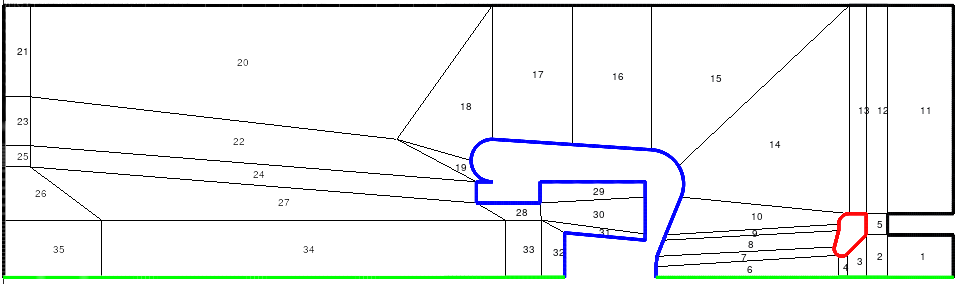
\includegraphics[width=\textwidth]{fig/geometry_v6}
   \end{subfigure}
   \begin{subfigure}{0.45\textwidth}
      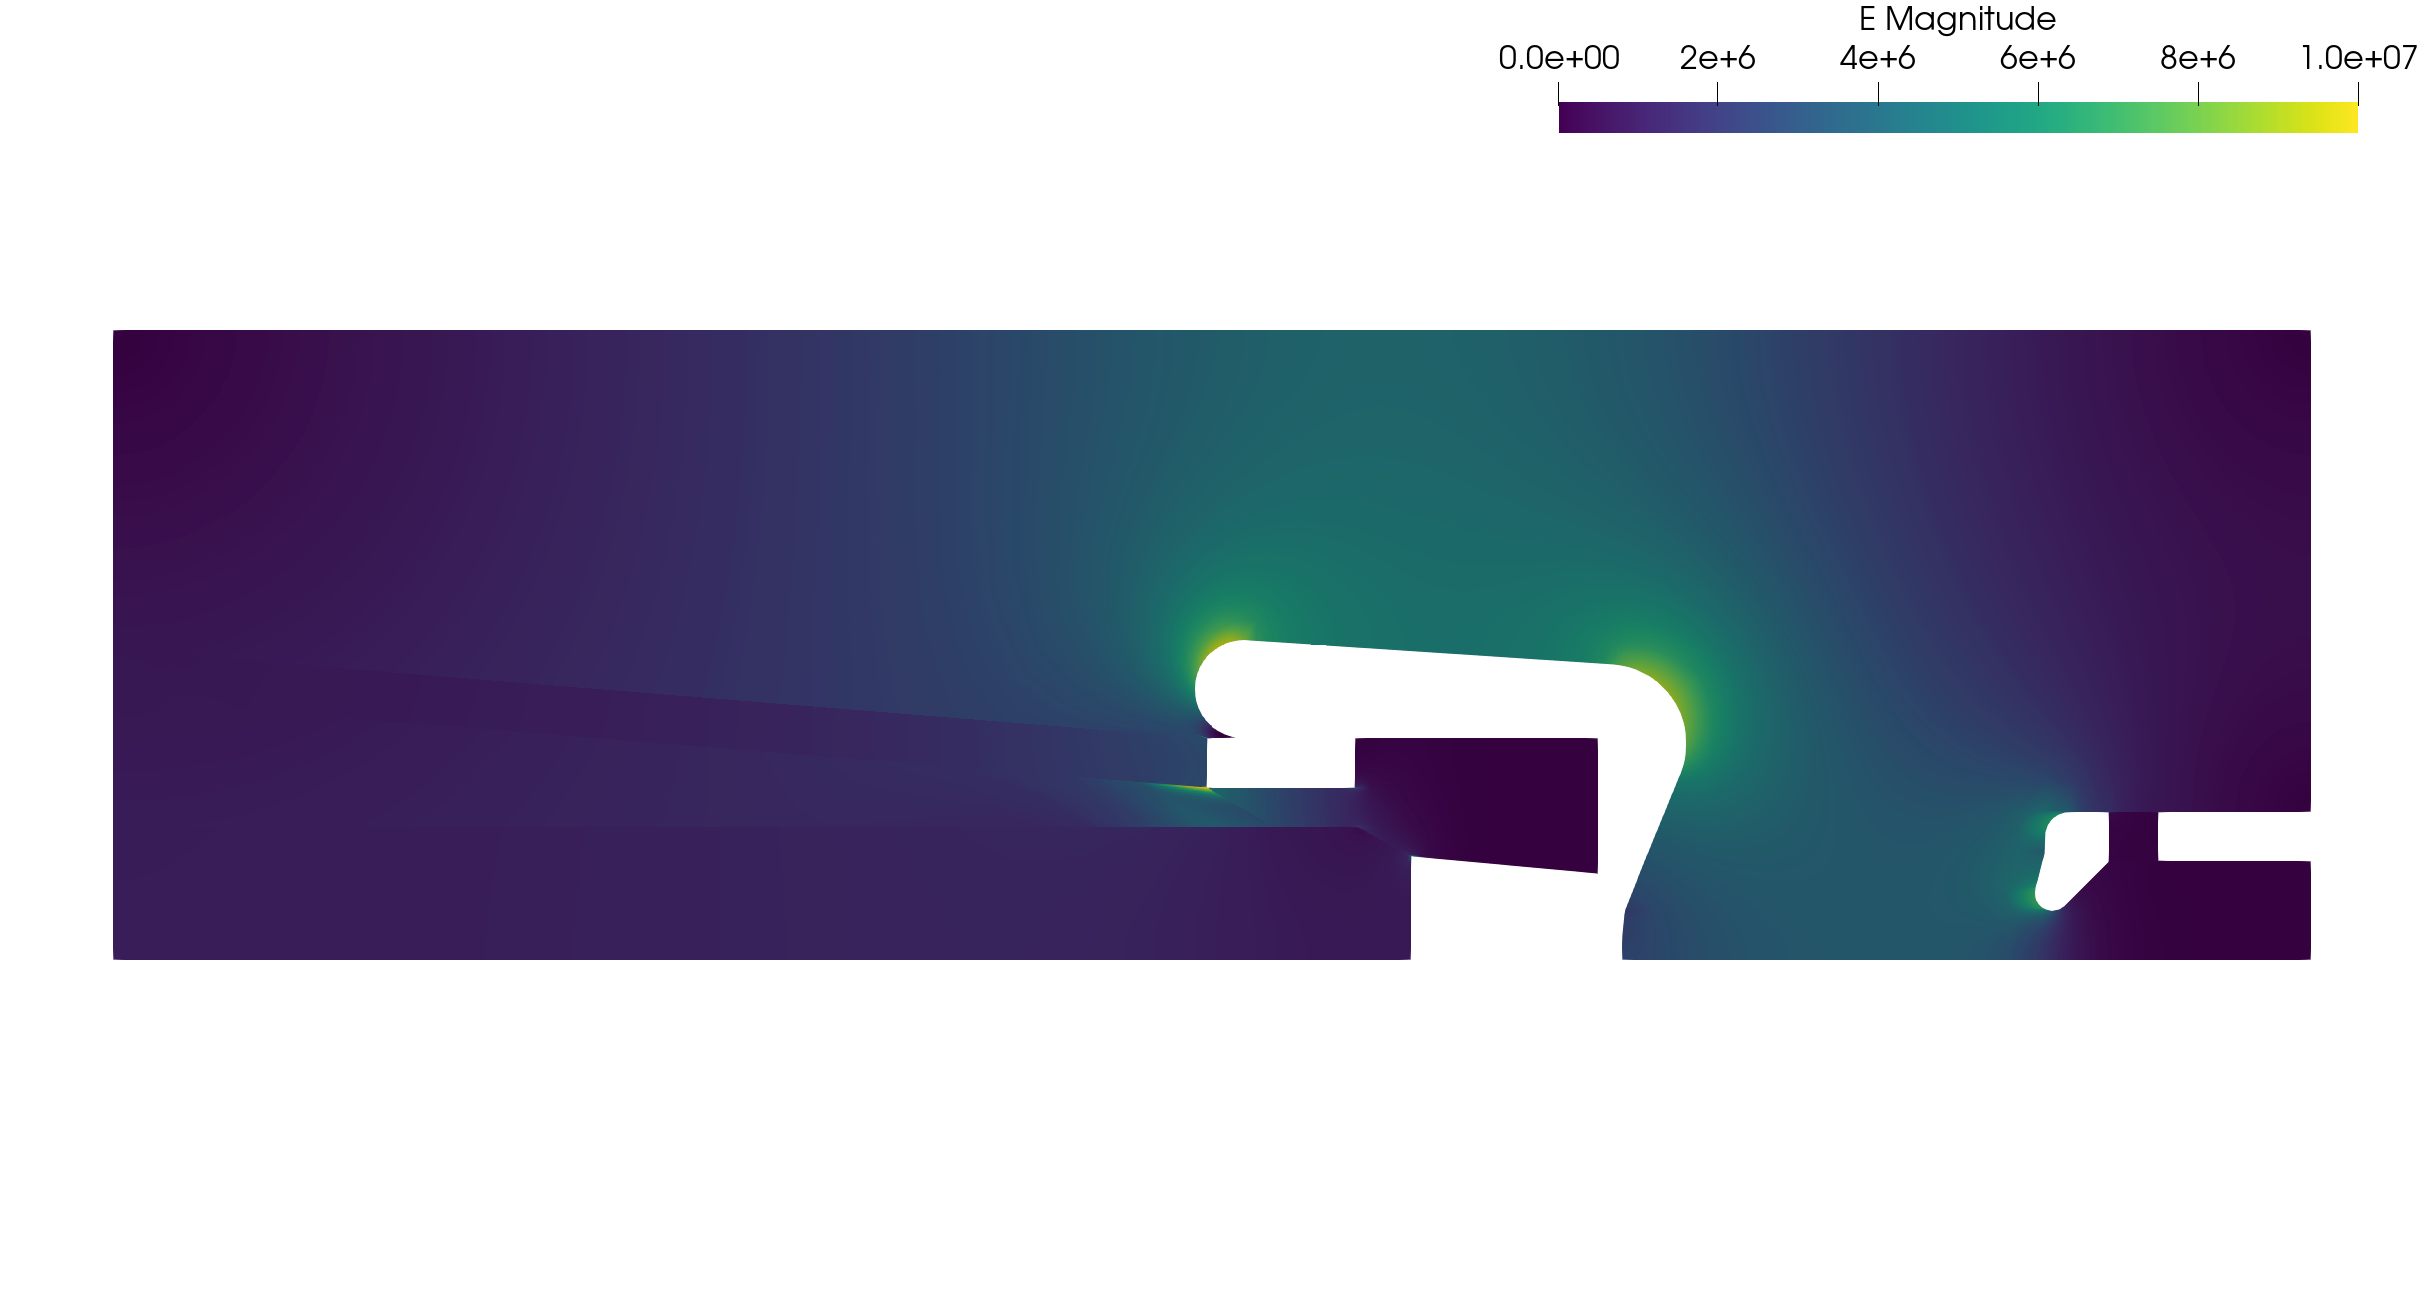
\includegraphics[width=\textwidth]{fig/E_v6}
   \end{subfigure}
   \caption{Initial geometry and magnitude of electric field.}
   \label{fig:init}
\end{figure}
\end{center}

\subsection{Optimization}
\begin{itemize}
   \item optimized geometry in Figure \ref{fig:opt}
   \item corresponding electric field for $p=3$, $n_\mathrm{sub}=16$, $V_\mathrm{el}=-300\ \mathrm{kV}$ and $V_\mathrm{ar}=1\ \mathrm{kV}$
   \item cost function employs $I = \{ 14, \dots, 19 \}$
   \item \textbf{results}: \qquad
                           \begin{tabular}{c|c|c|c}
                              & $(V_\mathrm{el}-625)\ \mathrm{in}\ \mathrm{cm}^3$ & $\frac{1}{|I|} \sum_{i \in I} \max_{\mathbf{x} \in \Omega_i} \| \mathbf{E}(\mathbf{x}) \|_2\ \mathrm{in}\ \frac{\mathrm{MV}}{\mathrm{m}}$ & $\max_{\mathbf{x} \in \Omega} \| \mathbf{E}(\mathbf{x}) \|_2\ \mathrm{in}\ \frac{\mathrm{MV}}{\mathrm{m}}$ \\
                              \hline
                              initial & 2.458 & 7.858 & 9.272 \\
                              optimized & -55.532 & 6.625 & 7.318 \\
                            \end{tabular}
\end{itemize}

\begin{center}
\begin{figure}[H]
   \begin{subfigure}{0.45\textwidth}
      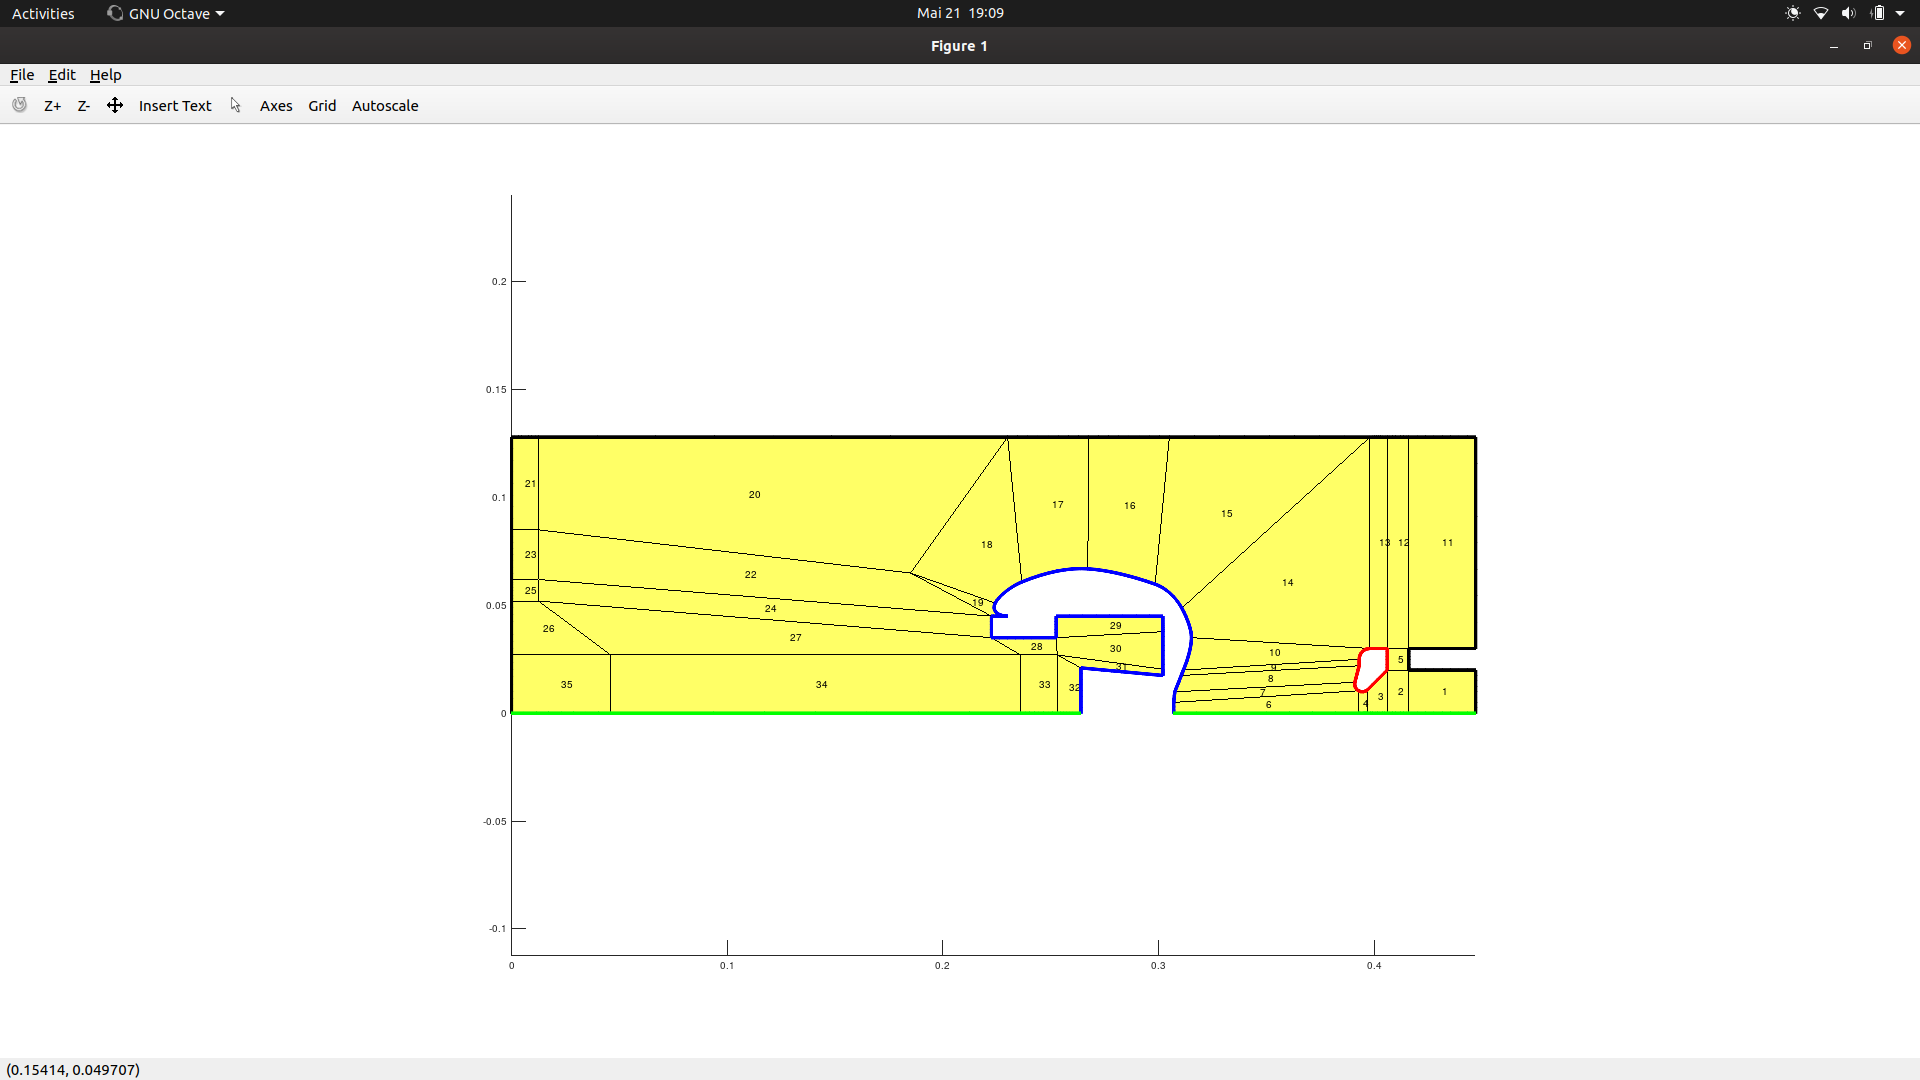
\includegraphics[width=\textwidth]{fig/geometry_v6_opt_order=3_run2}
   \end{subfigure}
   \begin{subfigure}{0.45\textwidth}
      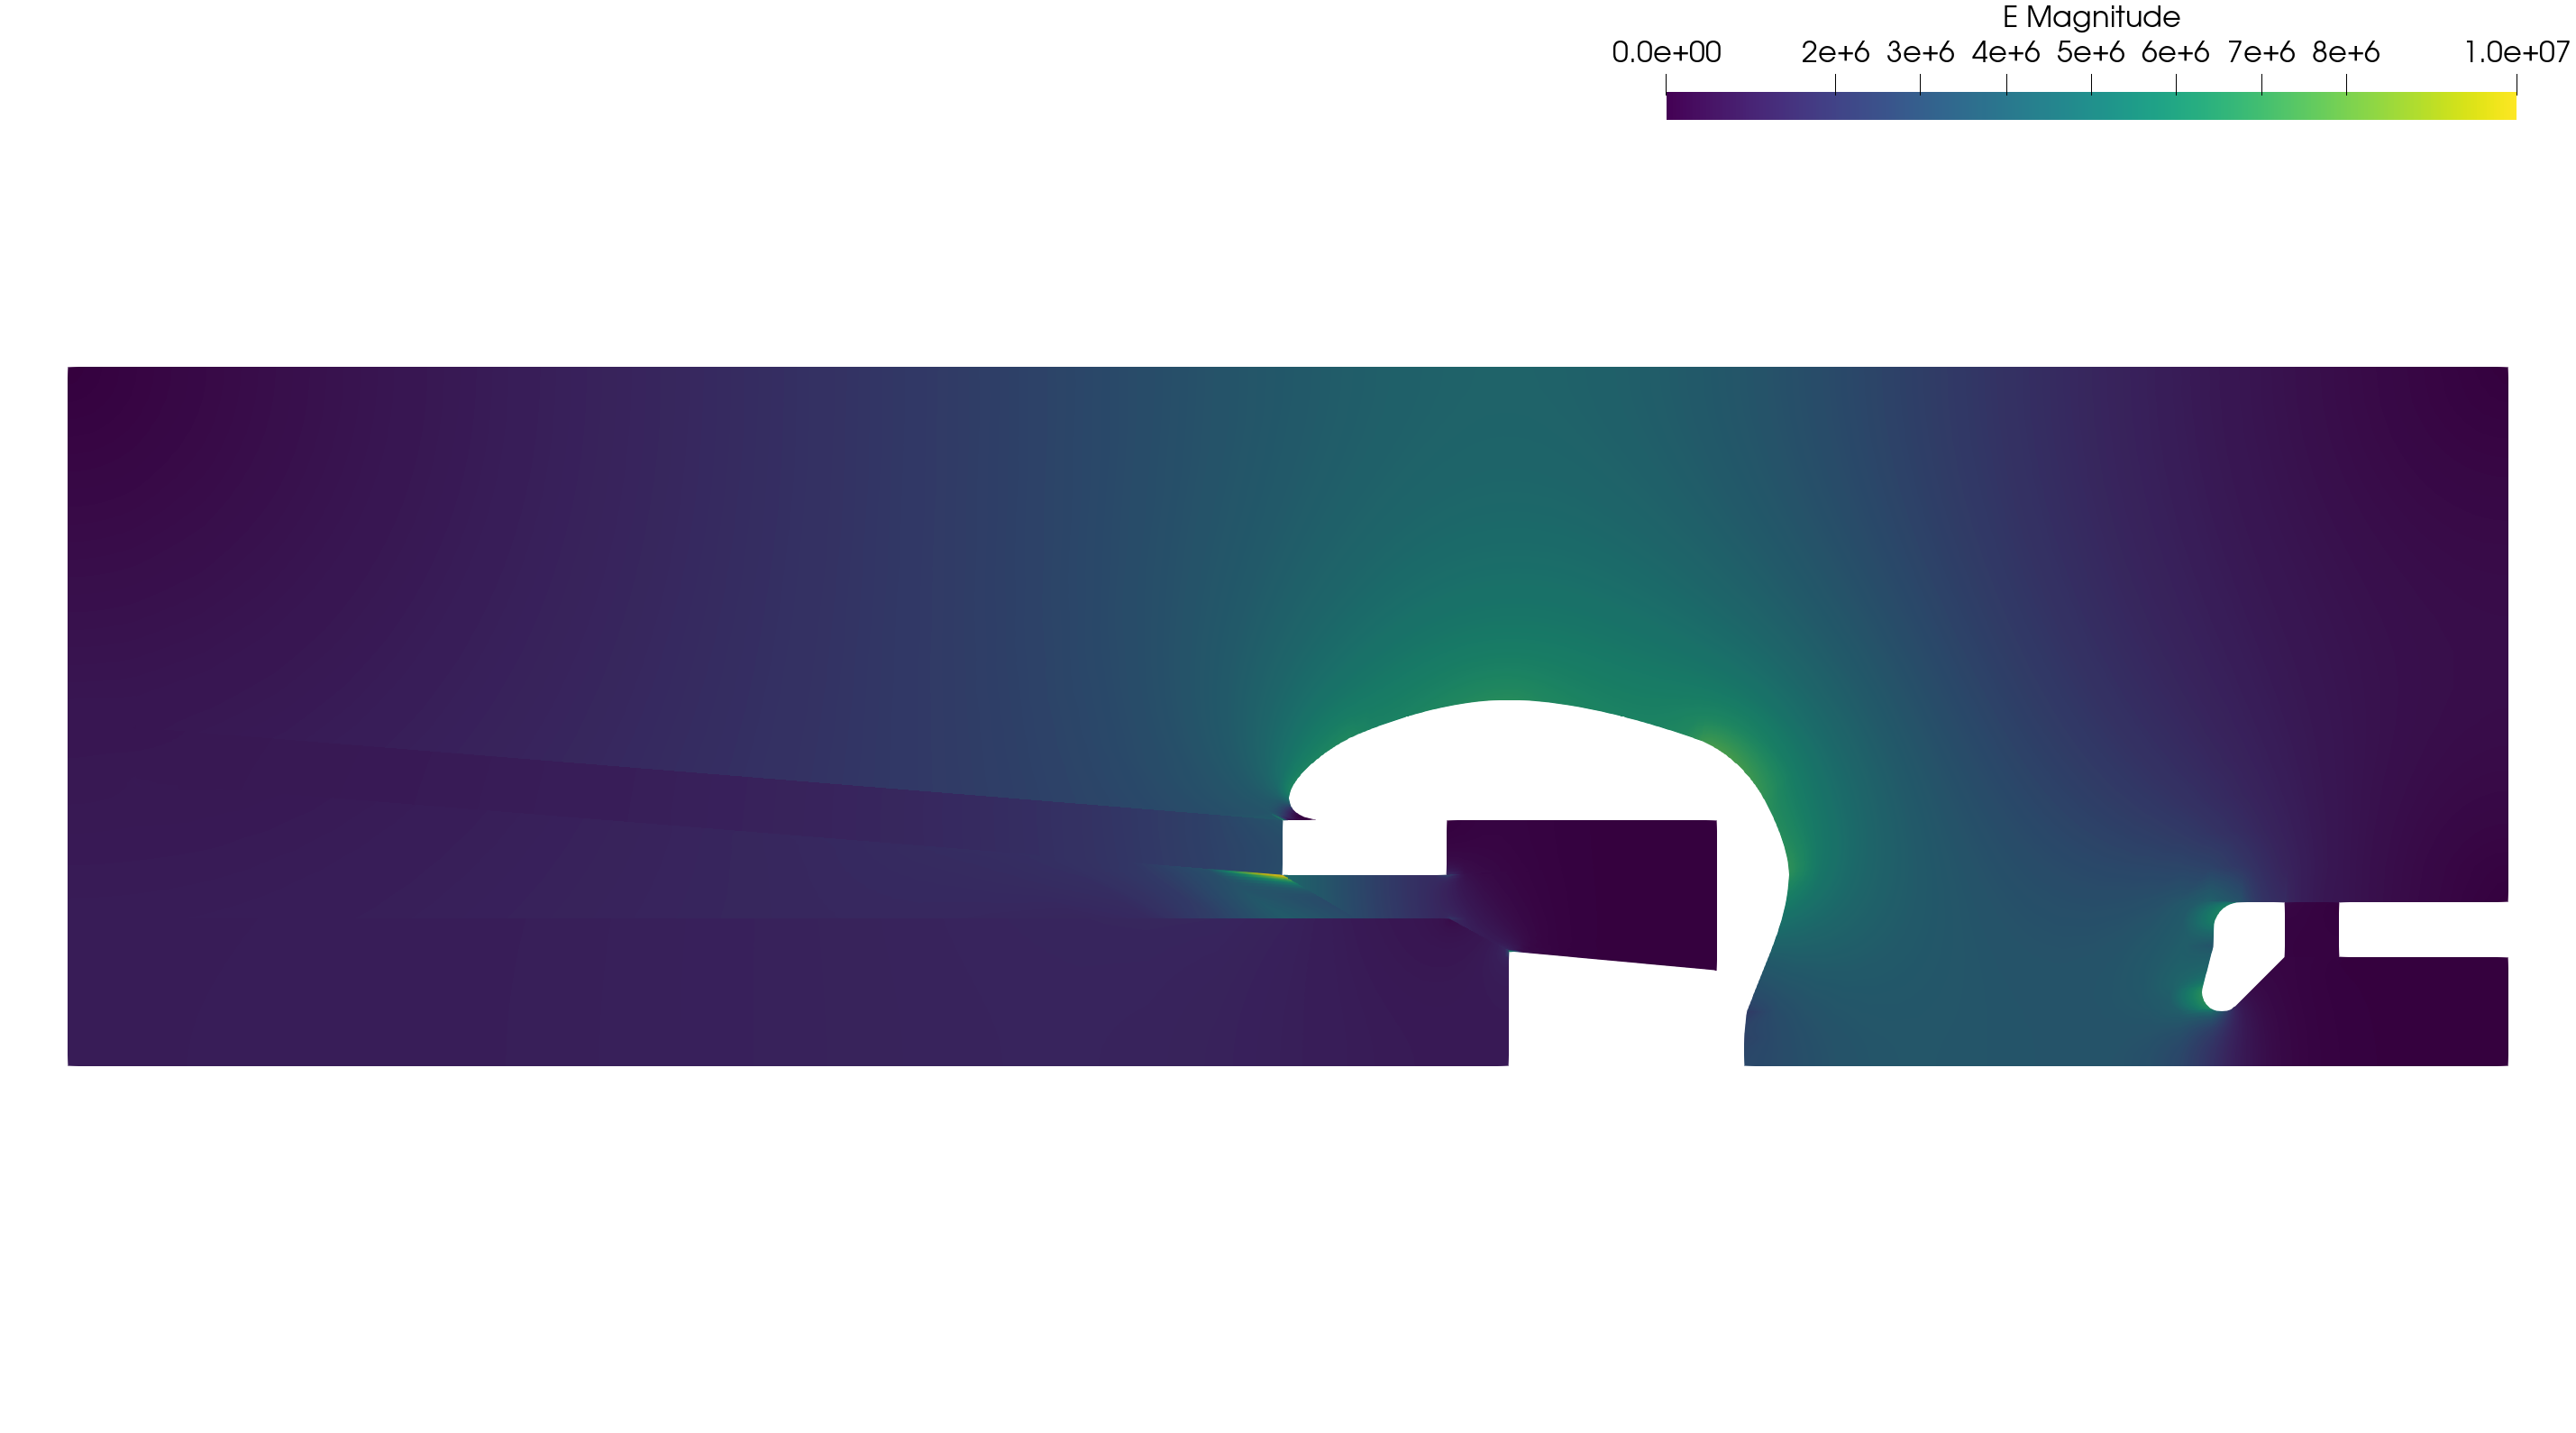
\includegraphics[width=\textwidth]{fig/E_v6_opt_order=3_run2}
   \end{subfigure}
   \caption{Optimized geometry and electric field.}
   \label{fig:opt}
\end{figure}
\end{center}

\newpage

\subsection{Tracking}
\begin{itemize}
   \item \textbf{general settings}: $Q=100\ \mathrm{fC}$
   \item \textbf{spatial distribution}: see Figure \ref{fig:gen_sp} for distribution generated from measurement and for comparison with laser measurement
   \item see Figure \ref{fig:gen_tmp} for spatial distribution from Gaussian ($\sigma=400\ \mu \mathrm{m}$)
   \item \textbf{temporal distribution}: Gaussian with $\sigma=5\ \mathrm{ps}$\ (is measurement data available?)
\end{itemize}

\begin{center}
\begin{figure}[H]
   \begin{subfigure}{0.4\textwidth}
      \begin{tikzpicture}
   \begin{axis}[
      axis equal,
      try min ticks=6,
      max space between ticks=1000pt,
      enlargelimits=true,
      xlabel=$x\ \mathrm{in}\ \mathrm{mm}$,
      ylabel=$y\ \mathrm{in}\ \mathrm{mm}$,
      ]

      \addplot[color=TUDa-1a, only marks, mark=*] table {fig/astra/gen/laser_I=2048_Q=0.0001_sc=0.005_gen.dat};
      \addplot[color=TUDa-1a, only marks, mark=*] table {fig/astra/gen/laser_I=2048_Q=0.0001_sc=0.005_probe.dat};
      % \addplot[color=TUDa-9a, only marks, mark=*] table {fig/astra/gen/laser_I=1024_Q=0.0001_sc=0.005_probe.dat};

   \end{axis}
\end{tikzpicture}

   \end{subfigure}
   \qquad \qquad \qquad
   \begin{subfigure}{0.5\textwidth}
      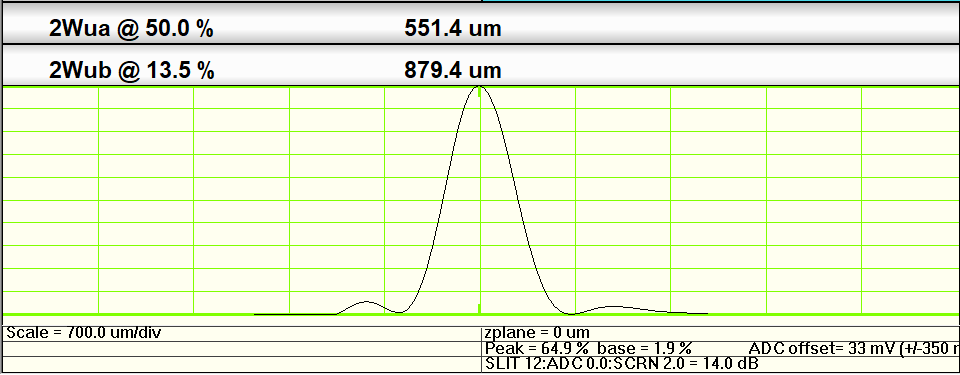
\includegraphics[width=\textwidth]{fig/laser}
   \end{subfigure}
   \caption{Spatial distribution generated from measurement ($2^{11}$ particles) and laser measurement.}
   \label{fig:gen_sp}
\end{figure}
\end{center}

\begin{center}
\begin{figure}[H]
   \begin{subfigure}{0.4\textwidth}
      \begin{tikzpicture}
   \begin{axis}[
      axis equal,
      try min ticks=6,
      max space between ticks=1000pt,
      enlargelimits=true,
      xlabel=$x\ \mathrm{in}\ \mathrm{mm}$,
      ylabel=$y\ \mathrm{in}\ \mathrm{mm}$,
      ]

      \addplot[color=TUDa-1a, only marks, mark=*] table {fig/astra/gen/I=1024_Q=0.0001_sc=0.005_gen.dat};
      \addplot[color=TUDa-1a, only marks, mark=*] table {fig/astra/gen/I=1024_Q=0.0001_sc=0.005_probe.dat};
      % \addplot[color=TUDa-9a, only marks, mark=*] table {fig/astra/gen/laser_I=1024_Q=0.0001_sc=0.005_probe.dat};

   \end{axis}
\end{tikzpicture}

   \end{subfigure}
   \qquad \qquad \qquad
   \begin{subfigure}{0.4\textwidth}
      \begin{tikzpicture}
   \begin{axis}[
      try min ticks=6,
      max space between ticks=1000pt,
      enlargelimits=true,
      xlabel=$t\ \mathrm{in\ ps}$,
      ylabel=$N_\mathrm{part}$,
      ]

      \addplot[color=TUDa-1a, ultra thick] table {fig/astra/gen/laser_I=2048_Q=0.0001_sc=0.005_tmp.dat};

   \end{axis}
\end{tikzpicture}

   \end{subfigure}
   \caption{Spatial distribution from Gaussian ($\sigma=400\ \mu \mathrm{m}$, $2^{10}$ particles) and temporal distribution ($2^{11}$ particles).}
   \label{fig:gen_tmp}
\end{figure}
\end{center}

\newpage

\begin{itemize}
   \item \textbf{convergence of time integrator}: relative error of normalized transverse emmitance $\epsilon$ w.\,r.\,t.\ finest time step is shown in Figure \ref{fig:int_cvg}
   \item computed with $n_x=n_y=8$ ($h_x=h_y=1.875 \cdot 10^{-4}$) and $n_z=256$ ($h_z=4.258 \cdot 10^{-4}$)
   \item $H=2^{-12}\ \mathrm{ns}$ used later on
\end{itemize}

\begin{center}
\begin{figure}[H]
   \begin{subfigure}{0.4\textwidth}
      \begin{tikzpicture}
   \begin{axis}[
      axis equal,
      try min ticks=4,
      max space between ticks=1000pt,
      enlargelimits=true,
      xlabel=$z / \mathrm{m}$,
      ylabel=$\epsilon / \mathrm{mrad\ mm}$,
      ]

      \addplot[color=TUDa-1a] table {fig/astra/int/photogun_int_emit_H_it=-13.dat};
      \addlegendentry{$H=2^{-13}$}
      \addplot[color=TUDa-2a] table {fig/astra/int/photogun_int_emit_H_it=-12.dat};
      \addlegendentry{$H=2^{-12}$}
      \addplot[color=TUDa-3a] table {fig/astra/int/photogun_int_emit_H_it=-11.dat};
      \addlegendentry{$H=2^{-11}$}
      \addplot[color=TUDa-4a] table {fig/astra/int/photogun_int_emit_H_it=-10.dat};
      \addlegendentry{$H=2^{-10}$}
      \addplot[color=TUDa-5a] table {fig/astra/int/photogun_int_emit_H_it=-9.dat};
      \addlegendentry{$H=2^{-9}$}
      \addplot[color=TUDa-6a] table {fig/astra/int/photogun_int_emit_H_it=-8.dat};
      \addlegendentry{$H=2^{-8}$}

   \end{axis}
\end{tikzpicture}

   \end{subfigure}
   \qquad \qquad \qquad
   \begin{subfigure}{0.4\textwidth}
      \begin{tikzpicture}
   \begin{loglogaxis}[
      axis equal,
      try min ticks=4,
      max space between ticks=1000pt,
      enlargelimits=true,
      xlabel=$H / \mathrm{ns}$,
      ylabel=$\|\Delta \epsilon\|_\infty / \mathrm{mrad\ mm}$,
      ]

      \addplot[color=TUDa-1a, ultra thick] table {fig/astra/int/photogun_int_err.dat};

   \end{loglogaxis}
\end{tikzpicture}

   \end{subfigure}
   \caption{Normalized transverse emmitance and relative error in $l_\infty$-norm.}
   \label{fig:int_cvg}
\end{figure}
\end{center}

\newpage

\begin{itemize}
   \item \textbf{convergence of field map}: look at convergence with number of grid points in transverse $(n_x, n_y)$ and longitudinal $(n_z)$ direction individually
   \item Figure \ref{fig:map_cvg_xy} looks at convergence of $n_x, n_y$ for $n_z=64$ ($h_z=1.703 \cdot 10^{-3}$)
   \item Figure \ref{fig:map_cvg_z} looks at convergence of $n_z$ for $n_x=n_y=8$ ($h_x=h_y=1.875 \cdot 10^{-4}$)
   \item $n_x=n_y=8$ ($h_x=h_y=1.875 \cdot 10^{-4}$) and $n_z=256$ ($h_z=4.258 \cdot 10^{-4}$) used for convergence studies later on
   \item $n_x=n_y=16$ ($h_x=h_y=2.5 \cdot 10^{-4}$) and $n_z=256$ ($h_z=4.258 \cdot 10^{-4}$) used for simulation later on (distribution from measurement is larger then that from Gaussian by more then a factor 2, see Figure \ref{fig:gen_sp} and Figure \ref{fig:gen_tmp})
\end{itemize}

\begin{center}
\begin{figure}[H]
   \begin{subfigure}{0.4\textwidth}
      \begin{tikzpicture}
   \begin{axis}[
      axis equal,
      try min ticks=4,
      max space between ticks=1000pt,
      enlargelimits=true,
      xlabel=$z / \mathrm{m}$,
      ylabel=$\epsilon / \mathrm{mrad\ mm}$,
      ]

      \addplot[color=TUDa-1a] table {fig/astra/map/photogun_map_emit_nx=ny=8_nz=64.dat};
      \addlegendentry{$n_x=8$}
      \addplot[color=TUDa-2a] table {fig/astra/map/photogun_map_emit_nx=ny=16_nz=64.dat};
      \addlegendentry{$n_x=16$}
      \addplot[color=TUDa-3a] table {fig/astra/map/photogun_map_emit_nx=ny=32_nz=64.dat};
      \addlegendentry{$n_x=32$}
      \addplot[color=TUDa-4a] table {fig/astra/map/photogun_map_emit_ref_nx=ny=64_nz=64.dat};
      \addlegendentry{$n_x=64$}

   \end{axis}
\end{tikzpicture}

   \end{subfigure}
   \qquad \qquad \qquad
   \begin{subfigure}{0.4\textwidth}
      \begin{tikzpicture}
   \begin{loglogaxis}[
      axis equal,
      try min ticks=4,
      max space between ticks=1000pt,
      enlargelimits=true,
      xlabel=$n_x$,
      ylabel=$\|\Delta \epsilon\|_\infty / \mathrm{mrad\ mm}$,
      ]

      \addplot[color=TUDa-1a, ultra thick] table {fig/astra/map/photogun_map_err_nz=64.dat};

   \end{loglogaxis}
\end{tikzpicture}

   \end{subfigure}
   \caption{Normalized transverse emmitance and relative error in $l_\infty$-norm for $n_z=64$ ($h_z=1.703 \cdot 10^{-3}$) and $n_x=n_y$ variable.}
   \label{fig:map_cvg_xy}
\end{figure}
\end{center}

\begin{center}
\begin{figure}[H]
   \begin{subfigure}{0.4\textwidth}
      \begin{tikzpicture}
   \begin{axis}[
      axis equal,
      try min ticks=4,
      max space between ticks=1000pt,
      enlargelimits=true,
      xlabel=$z\ \mathrm{in\ m}$,
      ylabel=$\epsilon\ \mathrm{in\ mrad\ mm}$,
      ]

      \addplot[color=TUDa-1a] table {fig/astra/map/nz/photogun_map_emit_nx=ny=8_nz=16.dat};
      \addlegendentry{$n_z=16$}
      \addplot[color=TUDa-2a] table {fig/astra/map/nz/photogun_map_emit_nx=ny=8_nz=32.dat};
      \addlegendentry{$n_x=32$}
      \addplot[color=TUDa-3a] table {fig/astra/map/nz/photogun_map_emit_nx=ny=8_nz=64.dat};
      \addlegendentry{$n_x=64$}
      \addplot[color=TUDa-4a] table {fig/astra/map/nz/photogun_map_emit_nx=ny=8_nz=128.dat};
      \addlegendentry{$n_x=128$}
      \addplot[color=TUDa-5a] table {fig/astra/map/nz/photogun_map_emit_nx=ny=8_nz=256.dat};
      \addlegendentry{$n_x=256$}
      \addplot[color=TUDa-6a] table {fig/astra/map/nz/photogun_map_emit_ref_nx=ny=8_nz=512.dat};
      \addlegendentry{$n_x=512$}

   \end{axis}
\end{tikzpicture}

   \end{subfigure}
   \qquad \qquad \qquad
   \begin{subfigure}{0.4\textwidth}
      \begin{tikzpicture}
   \begin{loglogaxis}[
      try min ticks=4,
      max space between ticks=1000pt,
      enlargelimits=true,
      xlabel=$h_z\ \mathrm{in\ m}$,
      ylabel=$\mathrm{relative\ error\ in}\ l_\infty \mathrm{-norm}$,
      ]

      \addplot[color=TUDa-1a, ultra thick, mark=*] table {fig/astra/map/nz/photogun_map_err_nx=ny=8.dat};

   \end{loglogaxis}
\end{tikzpicture}

   \end{subfigure}
   \caption{Normalized transverse emmitance and relative error in $l_\infty$-norm for $n_z$ variable and $n_x=n_y=8$ ($h_x=h_y=1.875 \cdot 10^{-4}$).}
   \label{fig:map_cvg_z}
\end{figure}
\end{center}

\begin{itemize}
   \item \textbf{convergence of space charge}: look at convergence with number of grid cells in radial $(n_r)$ and longitudinal $(n_l)$ direction and number of particles $(n_I)$ separately

   \item Figure \ref{fig:sc_cvg_rl} looks at convergence of $n_r, n_l$ for $n_I=2^{10}$
   \item $n_r=n_l=64$ ($h_r=2.344 \cdot 10^{-5}, h_l=1.703 \cdot 10^{-3}$) used later on

   \item Figure \ref{fig:sc_cvg_I} looks at convergence of $n_I$ for $n_r=n_l=64$ ($h_r=2.344 \cdot 10^{-5}, h_l=1.703 \cdot 10^{-3}$)
   \item $n_I=2^{11}$ used for simulation later on
\end{itemize}

\begin{center}
\begin{figure}[H]
   \begin{subfigure}{0.4\textwidth}
      \begin{tikzpicture}
   \begin{axis}[
      axis equal,
      try min ticks=4,
      max space between ticks=1000pt,
      enlargelimits=true,
      xlabel=$z / \mathrm{m}$,
      ylabel=$\epsilon / \mathrm{mrad\ mm}$,
      legend style={fill=none}
      ]

      \addplot[color=TUDa-6a] table {fig/astra/sc/nr_nl/photogun_sc_emit_ref_nI=1024_nr=64_nc=2_nl=64.dat};
      \addlegendentry{$n_r=64\ n_l=64$}

      \addplot[color=TUDa-5a] table {fig/astra/sc/nr_nl/photogun_sc_emit_ref_nI=1024_nr=32_nc=2_nl=32.dat};
      \addlegendentry{$n_r=32\ n_l=32$}

      \addplot[color=TUDa-1a] table {fig/astra/sc/nr_nl/photogun_sc_emit_nI=1024_nr=4_nc=2_nl=4.dat};
      % \addlegendentry{$n_r=4\ n_l=4$}
      \addplot[color=TUDa-1a, dotted] table {fig/astra/sc/nr_nl/photogun_sc_emit_nI=1024_nr=4_nc=2_nl=8.dat};
      % \addlegendentry{$n_r=4\ n_l=8$}
      \addplot[color=TUDa-1a, dashed] table {fig/astra/sc/nr_nl/photogun_sc_emit_nI=1024_nr=4_nc=2_nl=16.dat};
      % \addlegendentry{$n_r=4\ n_l=16$}
      \addplot[color=TUDa-1a, dashdotted] table {fig/astra/sc/nr_nl/photogun_sc_emit_nI=1024_nr=4_nc=2_nl=32.dat};
      % \addlegendentry{$n_r=4\ n_l=32$}

      \addplot[color=TUDa-2a] table {fig/astra/sc/nr_nl/photogun_sc_emit_nI=1024_nr=8_nc=2_nl=4.dat};
      % \addlegendentry{$n_r=8\ n_l=4$}
      \addplot[color=TUDa-2a, dotted] table {fig/astra/sc/nr_nl/photogun_sc_emit_nI=1024_nr=8_nc=2_nl=8.dat};
      % \addlegendentry{$n_r=8\ n_l=8$}
      \addplot[color=TUDa-2a, dashed] table {fig/astra/sc/nr_nl/photogun_sc_emit_nI=1024_nr=8_nc=2_nl=16.dat};
      % \addlegendentry{$n_r=8\ n_l=16$}
      \addplot[color=TUDa-2a, dashdotted] table {fig/astra/sc/nr_nl/photogun_sc_emit_nI=1024_nr=8_nc=2_nl=32.dat};
      % \addlegendentry{$n_r=8\ n_l=32$}

      \addplot[color=TUDa-3a] table {fig/astra/sc/nr_nl/photogun_sc_emit_nI=1024_nr=16_nc=2_nl=4.dat};
      % \addlegendentry{$n_r=16\ n_l=4$}
      \addplot[color=TUDa-3a, dotted] table {fig/astra/sc/nr_nl/photogun_sc_emit_nI=1024_nr=16_nc=2_nl=8.dat};
      % \addlegendentry{$n_r=16\ n_l=8$}
      \addplot[color=TUDa-3a, dashed] table {fig/astra/sc/nr_nl/photogun_sc_emit_nI=1024_nr=16_nc=2_nl=16.dat};
      % \addlegendentry{$n_r=16\ n_l=16$}
      \addplot[color=TUDa-3a, dashdotted] table {fig/astra/sc/nr_nl/photogun_sc_emit_nI=1024_nr=16_nc=2_nl=32.dat};
      % \addlegendentry{$n_r=16\ n_l=32$}

      \addplot[color=TUDa-4a] table {fig/astra/sc/nr_nl/photogun_sc_emit_nI=1024_nr=32_nc=2_nl=4.dat};
      % \addlegendentry{$n_r=32\ n_l=4$}
      \addplot[color=TUDa-4a, dotted] table {fig/astra/sc/nr_nl/photogun_sc_emit_nI=1024_nr=32_nc=2_nl=8.dat};
      % \addlegendentry{$n_r=32\ n_l=8$}
      \addplot[color=TUDa-4a, dashed] table {fig/astra/sc/nr_nl/photogun_sc_emit_nI=1024_nr=32_nc=2_nl=16.dat};
      % \addlegendentry{$n_r=32\ n_l=16$}

   \end{axis}
\end{tikzpicture}

   \end{subfigure}
   \qquad \qquad \qquad
   \begin{subfigure}{0.4\textwidth}
      \begin{tikzpicture}
   \begin{loglogaxis}[
      try min ticks=4,
      max space between ticks=1000pt,
      enlargelimits=true,
      xlabel=$n_l$,
      ylabel=$\|\Delta \epsilon\|_\infty / \mathrm{mrad\ mm}$,
      ]

      \addplot[color=TUDa-1a, ultra thick] table {fig/astra/sc/nr_nl/photogun_sc_err_nI=1024_nr=4_nc=2.dat};
      \addlegendentry{$n_r=4$}
      \addplot[color=TUDa-2a, ultra thick] table {fig/astra/sc/nr_nl/photogun_sc_err_nI=1024_nr=8_nc=2.dat};
      \addlegendentry{$n_r=8$}
      \addplot[color=TUDa-3a, ultra thick] table {fig/astra/sc/nr_nl/photogun_sc_err_nI=1024_nr=16_nc=2.dat};
      \addlegendentry{$n_r=16$}
      \addplot[color=TUDa-4a, ultra thick] table {fig/astra/sc/nr_nl/photogun_sc_err_nI=1024_nr=32_nc=2.dat};
      \addlegendentry{$n_r=32$}

   \end{loglogaxis}
\end{tikzpicture}

   \end{subfigure}
   \caption{Normalized transverse emmitance and relative error in $l_\infty$-norm for $n_I=2^{10}$ and $n_l, n_r$ variable.}
   \label{fig:sc_cvg_rl}
\end{figure}
\end{center}

\begin{center}
\begin{figure}[H]
   \begin{subfigure}{0.4\textwidth}
      \begin{tikzpicture}
   \begin{axis}[
      axis equal,
      try min ticks=4,
      max space between ticks=1000pt,
      enlargelimits=true,
      xlabel=$z / \mathrm{m}$,
      ylabel=$\epsilon / \mathrm{mrad\ mm}$,
      legend style={fill=none},
      legend pos=south east
      ]

      \addplot[color=TUDa-1a] table {fig/astra/sc/nI/photogun_sc_emit_nI=256_nr=16_nc=2_nl=16.dat};
      \addlegendentry{$n_I=2^{8}$}
      \addplot[color=TUDa-2a] table {fig/astra/sc/nI/photogun_sc_emit_nI=512_nr=16_nc=2_nl=16.dat};
      \addlegendentry{$n_I=2^{9}$}
      \addplot[color=TUDa-3a] table {fig/astra/sc/nI/photogun_sc_emit_nI=1024_nr=16_nc=2_nl=16.dat};
      \addlegendentry{$n_I=2^{10}$}
      \addplot[color=TUDa-4a] table {fig/astra/sc/nI/photogun_sc_emit_nI=2048_nr=16_nc=2_nl=16.dat};
      \addlegendentry{$n_I=2^{11}$}
      \addplot[color=TUDa-5a] table {fig/astra/sc/nI/photogun_sc_emit_nI=4096_nr=16_nc=2_nl=16.dat};
      \addlegendentry{$n_I=2^{12}$}

      \addplot[color=TUDa-6a] table {fig/astra/sc/nI/photogun_sc_emit_ref_nI=8192_nr=16_nc=2_nl=16.dat};
      \addlegendentry{$n_I=2^{13}$}

   \end{axis}
\end{tikzpicture}

   \end{subfigure}
   \qquad \qquad \qquad
   \begin{subfigure}{0.4\textwidth}
      \begin{tikzpicture}
   \begin{loglogaxis}[
      axis equal,
      try min ticks=4,
      max space between ticks=1000pt,
      enlargelimits=true,
      xlabel=$n_I$,
      ylabel=$\|\Delta \epsilon\|_\infty / \mathrm{mrad\ mm}$,
      ]

      \addplot[color=TUDa-1a, ultra thick] table {fig/astra/sc/nI/photogun_sc_err_nr=16_nc=2_nl=16.dat};

   \end{loglogaxis}
\end{tikzpicture}

   \end{subfigure}
   \caption{Normalized transverse emmitance and relative error in $l_\infty$-norm for $n_I$ variable and $n_r=n_l=64$ ($h_r=2.344 \cdot 10^{-5}, h_l=1.703 \cdot 10^{-3}$).}
   \label{fig:sc_cvg_I}
\end{figure}
\end{center}

% Cell_var
% \begin{center}
% \begin{figure}[H]
%    \begin{subfigure}{0.4\textwidth}
%       \begin{tikzpicture}
   \begin{axis}[
      axis equal,
      try min ticks=4,
      max space between ticks=1000pt,
      enlargelimits=true,
      xlabel=$z / \mathrm{m}$,
      ylabel=$\epsilon / \mathrm{mrad\ mm}$,
      legend style={fill=none}
      ]

      \addplot[color=TUDa-1a] table {fig/astra/sc/nc/photogun_sc_emit_nI=1024_nr=16_nc=0.5_nl=16.dat};
      \addlegendentry{$n_c=0.5$}
      \addplot[color=TUDa-2a] table {fig/astra/sc/nc/photogun_sc_emit_nI=1024_nr=16_nc=2_nl=16.dat};
      \addlegendentry{$n_c=2$}
      \addplot[color=TUDa-3a] table {fig/astra/sc/nc/photogun_sc_emit_ref_nI=1024_nr=16_nc=4_nl=16.dat};
      \addlegendentry{$n_c=4$}

   \end{axis}
\end{tikzpicture}

%    \end{subfigure}
%    \qquad \qquad \qquad
%    \begin{subfigure}{0.4\textwidth}
%       \begin{tikzpicture}
   \begin{loglogaxis}[
      axis equal,
      try min ticks=4,
      max space between ticks=1000pt,
      enlargelimits=true,
      xlabel=$n_c$,
      ylabel=$\mathrm{relative\ error\ in}\ l_\infty \mathrm{-norm}$,
      ]

      \addplot[color=TUDa-1a, ultra thick, mark=*] table {fig/astra/sc/nc/photogun_sc_err_nI=1024_nr=64_nl=64.dat};

   \end{loglogaxis}
\end{tikzpicture}

%    \end{subfigure}
%    \caption{Normalized transverse emmitance and relative error in $l_\infty$-norm for $n_I=2^{10}$ and $n_r=n_l=64$ ($h_r=2.344 \cdot 10^{-5}, h_l=1.703 \cdot 10^{-3}$).}
% \end{figure}
% \end{center}

\newpage

\begin{itemize}
   \item \textbf{tracking results}: simulation results for initial and optimized geometry
   \item continued tracking for $15\ \mathrm{cm}$ into the beam pipe
   \item initial normalized transverse emmitance for $H=2^{-12}$, $n_x=n_y=8$, $n_z=256$, $n_r=n_l=64$, $n_I=2^{11}$ and refined ($H=2^{-13}$, $n_x=n_y=16$, $n_z=512$, $n_r=n_l=128$, $n_I=2^{12}$) in Figure \ref{fig:res_eps} (uses Gaussian distribution, $\tilde{\epsilon}$ signifies refined solution)
   \item optimized normalized transverse emmitance for $H=2^{-12}$, $n_x=n_y=16$, $n_z=256$, $n_r=n_l=64$, $n_I=2^{11}$ also in Figure \ref{fig:res_eps} (uses distribution from measurement)
   \item rms beam size of initial geometry in Figure \ref{fig:res_init}
   \item rms beam size of optimized geometry in Figure \ref{fig:res_opt}
   \item \textbf{results}: \qquad
                           \begin{tabular}{c|c|c}
                              & $\mathrm{relative\ error\ of}\ \epsilon\ \mathrm{in}\ l_\infty \mathrm{-norm}$ & $\mathrm{relative\ error\ of}\ x_\mathrm{rms}\ \mathrm{in}\ l_\infty \mathrm{-norm}$ \\
                              \hline
                              $x$ & $3.38 \cdot 10^{-3}$ & $6.046 \cdot 10^{-3}$ \\
                              $y$ & $4.277 \cdot 10^{-3}$ & $1.027 \cdot 10^{-2}$ \\
                            \end{tabular}
\end{itemize}

\begin{center}
\begin{figure}[H]
   \begin{subfigure}{0.4\textwidth}
      \begin{tikzpicture}
   \begin{axis}[
      try min ticks=4,
      max space between ticks=1000pt,
      enlargelimits=true,
      xlabel=$z\ \mathrm{in\ m}$,
      ylabel=$\epsilon\ \mathrm{in\ mrad\ mm}$,
      legend style={fill=none},
      legend pos=south east
      ]

      \addplot[color=TUDa-1a] table {fig/astra/results/init/photogun_Xeps.dat};
      \addlegendentry{$\epsilon_x$}
      \addplot[color=TUDa-2a] table {fig/astra/results/init/photogun_Yeps.dat};
      \addlegendentry{$\epsilon_y$}

      \addplot[color=TUDa-3a] table {fig/astra/results/init/fine/photogun_Xeps.dat};
      \addlegendentry{$\tilde{\epsilon}_x$}
      \addplot[color=TUDa-4a] table {fig/astra/results/init/fine/photogun_Yeps.dat};
      \addlegendentry{$\tilde{\epsilon}_y$}
   \end{axis}
\end{tikzpicture}

   \end{subfigure}
   \qquad \qquad \qquad
   \begin{subfigure}{0.4\textwidth}
      \begin{tikzpicture}
   \begin{axis}[
      try min ticks=4,
      max space between ticks=1000pt,
      enlargelimits=true,
      xlabel=$z\ \mathrm{in\ m}$,
      ylabel=$\epsilon\ \mathrm{in\ mrad\ mm}$,
      legend style={fill=none}
      ]

      \addplot[color=TUDa-1a, thick] table {fig/astra/results/opt/photogun_Xeps.dat};
      \addlegendentry{$\epsilon_x$}
      \addplot[color=TUDa-2a, thick] table {fig/astra/results/opt/photogun_Yeps.dat};
      \addlegendentry{$\epsilon_y$}
   \end{axis}
\end{tikzpicture}

   \end{subfigure}
   \caption{Normalized transverse emmitance of initial and optimized geometry.}
   \label{fig:res_eps}
\end{figure}
\end{center}

\newpage

\begin{center}
\begin{figure}[H]
   \begin{subfigure}{0.4\textwidth}
      \begin{tikzpicture}
   \begin{axis}[
      axis equal,
      try min ticks=4,
      max space between ticks=1000pt,
      enlargelimits=true,
      xlabel=$z\ \mathrm{in\ m}$,
      ylabel=$10 \cdot x_\mathrm{rms}\ \mathrm{in\ m}$,
      legend style={fill=none}
      ]

      \addplot[color=TUDa-1a, thick] table[y expr=\thisrow{y}*0.01] {fig/astra/results/init/photogun_Xrms.dat};
      \addlegendentry{$x_\mathrm{rms}$}
      \addplot[color=TUDa-2a] table[y expr=\thisrow{y}*0.01] {fig/astra/results/init/photogun_Yrms.dat};
      \addlegendentry{$y_\mathrm{rms}$}

      \addplot[color=TUDa-3a] table[y expr=\thisrow{y}*0.01] {fig/astra/results/init/fine/photogun_Xrms.dat};
      \addlegendentry{$\tilde{x}_\mathrm{rms}$}
      \addplot[color=TUDa-4a] table[y expr=\thisrow{y}*0.01] {fig/astra/results/init/fine/photogun_Yrms.dat};
      \addlegendentry{$\tilde{y}_\mathrm{rms}$}

      % add geometry
      \addplot[color=TUDa-5a, semithick] table{fig/geometry/init/boundary11.dat};
      \addplot[color=black, semithick] table{fig/geometry/init/boundary12.dat};
      \addplot[color=TUDa-0b, semithick] table{fig/geometry/init/boundary13.dat};
      \addplot[color=black, semithick] table{fig/geometry/init/boundary14.dat};

      \addplot[color=TUDa-5a, semithick] table{fig/geometry/init/boundary21.dat};
      \addplot[color=TUDa-0b, semithick] table{fig/geometry/init/boundary22.dat};
      \addplot[color=TUDa-0b, semithick] table{fig/geometry/init/boundary23.dat};
      \addplot[color=TUDa-0b, semithick] table{fig/geometry/init/boundary24.dat};

      \addplot[color=TUDa-5a, semithick] table{fig/geometry/init/boundary31.dat};
      \addplot[color=TUDa-9a, semithick] table{fig/geometry/init/boundary32.dat};
      \addplot[color=TUDa-0b, semithick] table{fig/geometry/init/boundary33.dat};
      \addplot[color=TUDa-0b, semithick] table{fig/geometry/init/boundary34.dat};

      \addplot[color=TUDa-5a, semithick] table{fig/geometry/init/boundary41.dat};
      \addplot[color=TUDa-9a, semithick] table{fig/geometry/init/boundary42.dat};
      \addplot[color=TUDa-0b, semithick] table{fig/geometry/init/boundary43.dat};
      \addplot[color=TUDa-0b, semithick] table{fig/geometry/init/boundary44.dat};

      \addplot[color=TUDa-0b, semithick] table{fig/geometry/init/boundary51.dat};
      \addplot[color=TUDa-0b, semithick] table{fig/geometry/init/boundary52.dat};
      \addplot[color=TUDa-9a, semithick] table{fig/geometry/init/boundary53.dat};
      \addplot[color=black, semithick] table{fig/geometry/init/boundary54.dat};

      \addplot[color=TUDa-5a, semithick] table{fig/geometry/init/boundary61.dat};
      \addplot[color=TUDa-0b, semithick, opacity=0.35] table{fig/geometry/init/boundary62.dat};
      \addplot[color=TUDa-1a, semithick] table{fig/geometry/init/boundary63.dat};
      \addplot[color=TUDa-0b, semithick] table{fig/geometry/init/boundary64.dat};

      \addplot[color=TUDa-0b, semithick] table{fig/geometry/init/boundary71.dat};
      \addplot[color=TUDa-0b, semithick] table{fig/geometry/init/boundary72.dat};
      \addplot[color=TUDa-1a, semithick] table{fig/geometry/init/boundary73.dat};
      \addplot[color=TUDa-9a, semithick] table{fig/geometry/init/boundary74.dat};

      \addplot[color=TUDa-0b, semithick] table{fig/geometry/init/boundary81.dat};
      \addplot[color=TUDa-0b, semithick] table{fig/geometry/init/boundary82.dat};
      \addplot[color=TUDa-1a, semithick] table{fig/geometry/init/boundary83.dat};
      \addplot[color=TUDa-9a, semithick] table{fig/geometry/init/boundary84.dat};

      \addplot[color=TUDa-0b, semithick] table{fig/geometry/init/boundary91.dat};
      \addplot[color=TUDa-0b, semithick] table{fig/geometry/init/boundary92.dat};
      \addplot[color=TUDa-1a, semithick] table{fig/geometry/init/boundary93.dat};
      \addplot[color=TUDa-9a, semithick] table{fig/geometry/init/boundary94.dat};

      \addplot[color=TUDa-0b, semithick] table{fig/geometry/init/boundary101.dat};
      \addplot[color=TUDa-0b, semithick] table{fig/geometry/init/boundary102.dat};
      \addplot[color=TUDa-1a, semithick] table{fig/geometry/init/boundary103.dat};
      \addplot[color=TUDa-9a, semithick] table{fig/geometry/init/boundary104.dat};

      \addplot[color=black, semithick] table{fig/geometry/init/boundary111.dat};
      \addplot[color=black, semithick] table{fig/geometry/init/boundary112.dat};
      \addplot[color=TUDa-0b, semithick] table{fig/geometry/init/boundary113.dat};
      \addplot[color=black, semithick] table{fig/geometry/init/boundary114.dat};

      \addplot[color=TUDa-0b, semithick] table{fig/geometry/init/boundary121.dat};
      \addplot[color=black, semithick] table{fig/geometry/init/boundary122.dat};
      \addplot[color=TUDa-0b, semithick] table{fig/geometry/init/boundary123.dat};
      \addplot[color=TUDa-0b, semithick] table{fig/geometry/init/boundary124.dat};

      \addplot[color=TUDa-9a, semithick] table{fig/geometry/init/boundary131.dat};
      \addplot[color=black, semithick] table{fig/geometry/init/boundary132.dat};
      \addplot[color=TUDa-0b, semithick] table{fig/geometry/init/boundary133.dat};
      \addplot[color=TUDa-0b, semithick] table{fig/geometry/init/boundary134.dat};

      \addplot[color=TUDa-0b, semithick] table{fig/geometry/init/boundary141.dat};
      \addplot[color=TUDa-0b, semithick] table{fig/geometry/init/boundary142.dat};
      \addplot[color=TUDa-1a, semithick] table{fig/geometry/init/boundary143.dat};
      \addplot[color=TUDa-0b, semithick] table{fig/geometry/init/boundary144.dat};

   \end{axis}
\end{tikzpicture}

   \end{subfigure}
   \qquad \qquad \qquad
   \begin{subfigure}{0.4\textwidth}
      \begin{tikzpicture}
   \begin{axis}[
      axis equal,
      try min ticks=4,
      max space between ticks=1000pt,
      enlargelimits=true,
      xlabel=$z\ \mathrm{in\ m}$,
      ylabel=$10 \cdot x_\mathrm{rms}\ \mathrm{in\ m}$,
      legend style={fill=none}
      ]

      \addplot[color=TUDa-1a, thick] table[y expr=\thisrow{y}*0.01] {fig/astra/results/init/photogun_Xrms.dat};
      \addlegendentry{$x_\mathrm{rms}$}
      \addplot[color=TUDa-2a] table[y expr=\thisrow{y}*0.01] {fig/astra/results/init/photogun_Yrms.dat};
      \addlegendentry{$y_\mathrm{rms}$}

      \addplot[color=TUDa-3a] table[y expr=\thisrow{y}*0.01] {fig/astra/results/init/fine/photogun_Xrms.dat};
      \addlegendentry{$\tilde{x}_\mathrm{rms}$}
      \addplot[color=TUDa-4a] table[y expr=\thisrow{y}*0.01] {fig/astra/results/init/fine/photogun_Yrms.dat};
      \addlegendentry{$\tilde{y}_\mathrm{rms}$}

      % add geometry
      \addplot[color=TUDa-5a, semithick] table{fig/geometry/init/boundary11.dat};
      \addplot[color=black, semithick] table{fig/geometry/init/boundary12.dat};
      \addplot[color=TUDa-0b, semithick] table{fig/geometry/init/boundary13.dat};
      \addplot[color=black, semithick] table{fig/geometry/init/boundary14.dat};

      \addplot[color=TUDa-5a, semithick] table{fig/geometry/init/boundary21.dat};
      \addplot[color=TUDa-0b, semithick] table{fig/geometry/init/boundary22.dat};
      \addplot[color=TUDa-0b, semithick] table{fig/geometry/init/boundary23.dat};
      \addplot[color=TUDa-0b, semithick] table{fig/geometry/init/boundary24.dat};

      \addplot[color=TUDa-5a, semithick] table{fig/geometry/init/boundary31.dat};
      \addplot[color=TUDa-9a, semithick] table{fig/geometry/init/boundary32.dat};
      \addplot[color=TUDa-0b, semithick] table{fig/geometry/init/boundary33.dat};
      \addplot[color=TUDa-0b, semithick] table{fig/geometry/init/boundary34.dat};

      \addplot[color=TUDa-5a, semithick] table{fig/geometry/init/boundary41.dat};
      \addplot[color=TUDa-9a, semithick] table{fig/geometry/init/boundary42.dat};
      \addplot[color=TUDa-0b, semithick] table{fig/geometry/init/boundary43.dat};
      \addplot[color=TUDa-0b, semithick] table{fig/geometry/init/boundary44.dat};

      \addplot[color=TUDa-0b, semithick] table{fig/geometry/init/boundary51.dat};
      \addplot[color=TUDa-0b, semithick] table{fig/geometry/init/boundary52.dat};
      \addplot[color=TUDa-9a, semithick] table{fig/geometry/init/boundary53.dat};
      \addplot[color=black, semithick] table{fig/geometry/init/boundary54.dat};

      \addplot[color=TUDa-5a, semithick] table{fig/geometry/init/boundary61.dat};
      \addplot[color=TUDa-0b, semithick, opacity=0.35] table{fig/geometry/init/boundary62.dat};
      \addplot[color=TUDa-1a, semithick] table{fig/geometry/init/boundary63.dat};
      \addplot[color=TUDa-0b, semithick] table{fig/geometry/init/boundary64.dat};

      \addplot[color=TUDa-0b, semithick] table{fig/geometry/init/boundary71.dat};
      \addplot[color=TUDa-0b, semithick] table{fig/geometry/init/boundary72.dat};
      \addplot[color=TUDa-1a, semithick] table{fig/geometry/init/boundary73.dat};
      \addplot[color=TUDa-9a, semithick] table{fig/geometry/init/boundary74.dat};

      \addplot[color=TUDa-0b, semithick] table{fig/geometry/init/boundary81.dat};
      \addplot[color=TUDa-0b, semithick] table{fig/geometry/init/boundary82.dat};
      \addplot[color=TUDa-1a, semithick] table{fig/geometry/init/boundary83.dat};
      \addplot[color=TUDa-9a, semithick] table{fig/geometry/init/boundary84.dat};

      \addplot[color=TUDa-0b, semithick] table{fig/geometry/init/boundary91.dat};
      \addplot[color=TUDa-0b, semithick] table{fig/geometry/init/boundary92.dat};
      \addplot[color=TUDa-1a, semithick] table{fig/geometry/init/boundary93.dat};
      \addplot[color=TUDa-9a, semithick] table{fig/geometry/init/boundary94.dat};

      \addplot[color=TUDa-0b, semithick] table{fig/geometry/init/boundary101.dat};
      \addplot[color=TUDa-0b, semithick] table{fig/geometry/init/boundary102.dat};
      \addplot[color=TUDa-1a, semithick] table{fig/geometry/init/boundary103.dat};
      \addplot[color=TUDa-9a, semithick] table{fig/geometry/init/boundary104.dat};

      \addplot[color=black, semithick] table{fig/geometry/init/boundary111.dat};
      \addplot[color=black, semithick] table{fig/geometry/init/boundary112.dat};
      \addplot[color=TUDa-0b, semithick] table{fig/geometry/init/boundary113.dat};
      \addplot[color=black, semithick] table{fig/geometry/init/boundary114.dat};

      \addplot[color=TUDa-0b, semithick] table{fig/geometry/init/boundary121.dat};
      \addplot[color=black, semithick] table{fig/geometry/init/boundary122.dat};
      \addplot[color=TUDa-0b, semithick] table{fig/geometry/init/boundary123.dat};
      \addplot[color=TUDa-0b, semithick] table{fig/geometry/init/boundary124.dat};

      \addplot[color=TUDa-9a, semithick] table{fig/geometry/init/boundary131.dat};
      \addplot[color=black, semithick] table{fig/geometry/init/boundary132.dat};
      \addplot[color=TUDa-0b, semithick] table{fig/geometry/init/boundary133.dat};
      \addplot[color=TUDa-0b, semithick] table{fig/geometry/init/boundary134.dat};

      \addplot[color=TUDa-0b, semithick] table{fig/geometry/init/boundary141.dat};
      \addplot[color=TUDa-0b, semithick] table{fig/geometry/init/boundary142.dat};
      \addplot[color=TUDa-1a, semithick] table{fig/geometry/init/boundary143.dat};
      \addplot[color=TUDa-0b, semithick] table{fig/geometry/init/boundary144.dat};

   \end{axis}
\end{tikzpicture}

   \end{subfigure}
   \caption{RMS beam size of initial geometry.}
   \label{fig:res_init}
\end{figure}
\end{center}

\begin{center}
\begin{figure}[H]
   \begin{subfigure}{0.4\textwidth}
      \begin{tikzpicture}
   \begin{axis}[
      try min ticks=4,
      max space between ticks=1000pt,
      enlargelimits=true,
      xlabel=$z\ \mathrm{in\ m}$,
      ylabel=$x_\mathrm{rms}\ \mathrm{in\ mm}$,
      legend style={fill=none}
      ]

      \addplot[color=TUDa-1a, thick] table {fig/astra/results/opt/photogun_Xrms.dat};
      \addlegendentry{$x_\mathrm{rms}$}
      \addplot[color=TUDa-2a, thick] table {fig/astra/results/opt/photogun_Yrms.dat};
      \addlegendentry{$y_\mathrm{rms}$}

   \end{axis}
\end{tikzpicture}

   \end{subfigure}
   \qquad \qquad \qquad
   \begin{subfigure}{0.4\textwidth}
      \begin{tikzpicture}
   \begin{axis}[
      axis equal,
      try min ticks=4,
      max space between ticks=1000pt,
      enlargelimits=true,
      xlabel=$z\ \mathrm{in\ m}$,
      ylabel=$10 \cdot x_\mathrm{rms}\ \mathrm{in\ m}$,
      legend style={fill=none}
      ]

      \addplot[color=TUDa-1a, thick] table[y expr=\thisrow{y}*0.01] {fig/astra/results/opt/photogun_Xrms.dat};
      \addlegendentry{$x_\mathrm{rms}$}
      \addplot[color=TUDa-2a, thick] table[y expr=\thisrow{y}*0.01] {fig/astra/results/opt/photogun_Yrms.dat};
      \addlegendentry{$y_\mathrm{rms}$}

      % add geometry
      \addplot[color=TUDa-5a, semithick] table{fig/geometry/opt/boundary11.dat};
      \addplot[color=black, semithick] table{fig/geometry/opt/boundary12.dat};
      \addplot[color=TUDa-0b, semithick] table{fig/geometry/opt/boundary13.dat};
      \addplot[color=black, semithick] table{fig/geometry/opt/boundary14.dat};

      \addplot[color=TUDa-5a, semithick] table{fig/geometry/opt/boundary21.dat};
      \addplot[color=TUDa-0b, semithick] table{fig/geometry/opt/boundary22.dat};
      \addplot[color=TUDa-0b, semithick] table{fig/geometry/opt/boundary23.dat};
      \addplot[color=TUDa-0b, semithick] table{fig/geometry/opt/boundary24.dat};

      \addplot[color=TUDa-5a, semithick] table{fig/geometry/opt/boundary31.dat};
      \addplot[color=TUDa-9a, semithick] table{fig/geometry/opt/boundary32.dat};
      \addplot[color=TUDa-0b, semithick] table{fig/geometry/opt/boundary33.dat};
      \addplot[color=TUDa-0b, semithick] table{fig/geometry/opt/boundary34.dat};

      \addplot[color=TUDa-5a, semithick] table{fig/geometry/opt/boundary41.dat};
      \addplot[color=TUDa-9a, semithick] table{fig/geometry/opt/boundary42.dat};
      \addplot[color=TUDa-0b, semithick] table{fig/geometry/opt/boundary43.dat};
      \addplot[color=TUDa-0b, semithick] table{fig/geometry/opt/boundary44.dat};

      \addplot[color=TUDa-0b, semithick] table{fig/geometry/opt/boundary51.dat};
      \addplot[color=TUDa-0b, semithick] table{fig/geometry/opt/boundary52.dat};
      \addplot[color=TUDa-9a, semithick] table{fig/geometry/opt/boundary53.dat};
      \addplot[color=black, semithick] table{fig/geometry/opt/boundary54.dat};

      \addplot[color=TUDa-5a, semithick] table{fig/geometry/opt/boundary61.dat};
      \addplot[color=TUDa-0b, semithick, opacity=0.35] table{fig/geometry/opt/boundary62.dat};
      \addplot[color=TUDa-1a, semithick] table{fig/geometry/opt/boundary63.dat};
      \addplot[color=TUDa-0b, semithick] table{fig/geometry/opt/boundary64.dat};

      \addplot[color=TUDa-0b, semithick] table{fig/geometry/opt/boundary71.dat};
      \addplot[color=TUDa-0b, semithick] table{fig/geometry/opt/boundary72.dat};
      \addplot[color=TUDa-1a, semithick] table{fig/geometry/opt/boundary73.dat};
      \addplot[color=TUDa-9a, semithick] table{fig/geometry/opt/boundary74.dat};

      \addplot[color=TUDa-0b, semithick] table{fig/geometry/opt/boundary81.dat};
      \addplot[color=TUDa-0b, semithick] table{fig/geometry/opt/boundary82.dat};
      \addplot[color=TUDa-1a, semithick] table{fig/geometry/opt/boundary83.dat};
      \addplot[color=TUDa-9a, semithick] table{fig/geometry/opt/boundary84.dat};

      \addplot[color=TUDa-0b, semithick] table{fig/geometry/opt/boundary91.dat};
      \addplot[color=TUDa-0b, semithick] table{fig/geometry/opt/boundary92.dat};
      \addplot[color=TUDa-1a, semithick] table{fig/geometry/opt/boundary93.dat};
      \addplot[color=TUDa-9a, semithick] table{fig/geometry/opt/boundary94.dat};

      \addplot[color=TUDa-0b, semithick] table{fig/geometry/opt/boundary101.dat};
      \addplot[color=TUDa-0b, semithick] table{fig/geometry/opt/boundary102.dat};
      \addplot[color=TUDa-1a, semithick] table{fig/geometry/opt/boundary103.dat};
      \addplot[color=TUDa-9a, semithick] table{fig/geometry/opt/boundary104.dat};

      \addplot[color=black, semithick] table{fig/geometry/opt/boundary111.dat};
      \addplot[color=black, semithick] table{fig/geometry/opt/boundary112.dat};
      \addplot[color=TUDa-0b, semithick] table{fig/geometry/opt/boundary113.dat};
      \addplot[color=black, semithick] table{fig/geometry/opt/boundary114.dat};

      \addplot[color=TUDa-0b, semithick] table{fig/geometry/opt/boundary121.dat};
      \addplot[color=black, semithick] table{fig/geometry/opt/boundary122.dat};
      \addplot[color=TUDa-0b, semithick] table{fig/geometry/opt/boundary123.dat};
      \addplot[color=TUDa-0b, semithick] table{fig/geometry/opt/boundary124.dat};

      \addplot[color=TUDa-9a, semithick] table{fig/geometry/opt/boundary131.dat};
      \addplot[color=black, semithick] table{fig/geometry/opt/boundary132.dat};
      \addplot[color=TUDa-0b, semithick] table{fig/geometry/opt/boundary133.dat};
      \addplot[color=TUDa-0b, semithick] table{fig/geometry/opt/boundary134.dat};

      \addplot[color=TUDa-0b, semithick] table{fig/geometry/opt/boundary141.dat};
      \addplot[color=TUDa-0b, semithick] table{fig/geometry/opt/boundary142.dat};
      \addplot[color=TUDa-1a, semithick] table{fig/geometry/opt/boundary143.dat};
      \addplot[color=TUDa-0b, semithick] table{fig/geometry/opt/boundary144.dat};

   \end{axis}
\end{tikzpicture}

   \end{subfigure}
   \caption{RMS beam size of optimized geometry.}
   \label{fig:res_opt}
\end{figure}
\end{center}
